\documentclass[12pt]{article}
\usepackage[utf8]{inputenc}
\usepackage[T1]{fontenc}
\usepackage{amsmath}
\usepackage{graphicx}

\title{Response to the first report on the article draft \emph{The
    Impact of Gas Bulk Rotation on the Lyman-$\alpha$ line.}} 
\author{Juan N. Garavito-Camargo, Jaime E. Forero-Romero, Mark Disjkstra}
\date{\today}

\begin{document}


\maketitle
We thank the referee for a detailed report. Indeed, the report
motivated us to explore a very important aspect of our results that we
had overlooked.  

We made a plot suggested by the referee that showed a clear
dependence of the line morphology with the viewing angle an effect
that we had deemed as negligeable after measuring a proxy statistic for
it (the integrated flux).

The correct interpretation is that, as the referee expected, there is
a strong effect on the morphology. 

This completely changed the focus of our paper. We have now completely
rewritten the Results and Discussion section in order to highlight
that result. We have also completeley dropped sections (e.g. the
asymetrical emission part) that obfuscate this main result.

In this document we address one by one the questions in the
report. However, we kindly ask the referee to revise directly the new
version of the paper, given the substantial changes from the first
version.


In what follows the comments by the referee are boldfaced.

Best regards, \\

The Authors\\




\section{Global Comments}

\subsection{Variation with the viewing angle}

{\bf The problematic of anisotropy is only studied from Sect3.4, the former
sections consider global quantities (spectral shapes, escape
fractions, etc...). This is ok only if there is NO anisotropy induced
by rotation, which is not obvious, a priori. You should make it clear
from the beginning, telling that you will investigate anisotropy at
the end of the paper only, because you checked that lya properties are
isotropic, at least in the range of parameters that you investigated
so far.}

As we mentioned in the introduction to this letter, there is indeed
an anisotropy in the line morphology. The paper was re-structured
accordingly.

However, the properties that we had measured as isotropic (integrated
flux and escape fracrion) remain anisotropic.


{\bf As explained in sect 3.4, rotation kills the spherical symmetry
  of your problem, and the rotation axis defines a preferential
  direction. We could expect some variation of the emerging flux, the
  lyman-alpha escape fraction, and the spectral shape, with viewing
  angle. From Fig8, it seems that the flux is the same in all
  directions for spherical distributions of sources. This important
  result is not enough emphasized.} 


We now emphasize in the abstract, section 3.2 and the conclusions the
result on the non-variation of the total flux with viewing angle.

{\bf Do you see any difference in the spectral shape with viewing
  angle? To illustrate this point, it would be interesting to build a
  2D plot as you did on Fig 5, but replace Nb scat in ordinates by the
  viewing angle $\mu$. We could immediatly see if there is an
  evolution of the shape with viewing angle or not. If you find NO
  evolution of the Lya shape with viewing angle, I think that it is an
  interesting counter-intuitive result, that you should advertise
  more.} 

As we metioned in the introduction to this reply, we prepared the
suggested plot and found strong variations of the spectral shape with
viewing angle. This result motivated us to re-structure the paper to
emphasize it.


{\bf What about the variation of lya escape fraction with viewing
  angle ? I propose that in the beginning of Sect.3 Results, you first
  emphasize that, maybe counter-intuitively, you did not find any
  variation of the Lya properties with viewing angle, so you will
  present first angle average lya properties, and you will come back
  to the anisotropy problematic only at the end on the paper.} 

We do not find any significant dependence of the escape fraction with
the viewing angle. This is shown in Figure \ref{escape_fraction} of this
document. We do not show this plot in the paper and only mention the
result at the beginning of Section 3.5.

\begin{figure}
\begin{center}
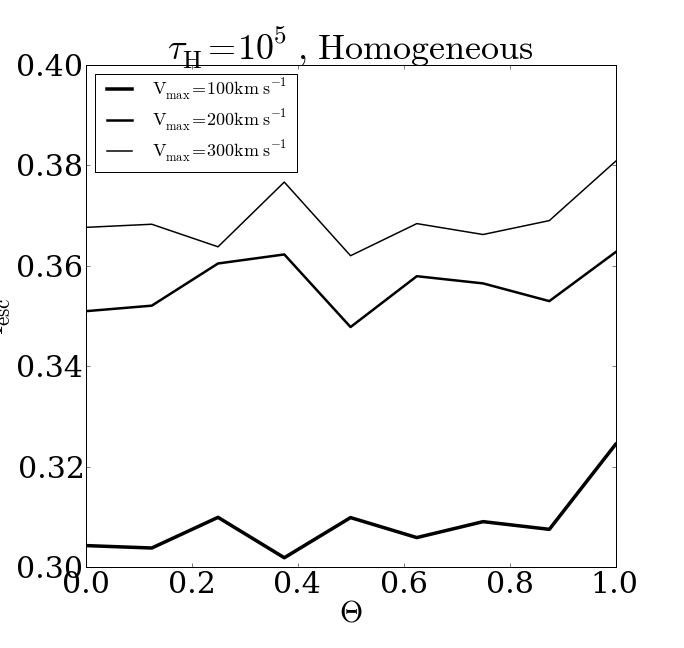
\includegraphics[scale=0.5]{escapefractionvstheta.png}
\end{center}
\caption{Escape Fraction as a function of $\mu$
\label{escape_fraction}}
\end{figure}


\section*{Outflow + Rotation}

{\bf So far, the model only includes rotation. However, most observed
  Lya spectra from LAEs, or even local galaxies, seem to be asymetric
  towards the red wavelengths, interpreted as a sign for outflows in
  these systems, often corroborated by others observables. Did you
  investigate how the rotation would modify the spectra emerging from
  expanding clouds?} 


We agree with the referee that this is an important point to study. 
We have not fully investigated it yet.  This is actually research
under development.   

\section*{Details}

\subsection*{Introduction}

{\bf With Orsi et al 2012, please cite also Garel et al 2012. With
  Zheng \& Wallace 2013, please cite also Behrens et al 2014.} 

Done.

\subsection*{Fig.1}

{\bf I guess that the spectra presented in Fig1 are integrated over
  all directions, right ? You should describe explicitly how you build
  them. You could skip the x notation in absciss, as it is not used in
  the discussion, whereas the velocity is used to compare to FWHM, on
  Fig2.} 

Now this figure is the Fig.4 in the paper. Given the depence on the
viewing angle we decided to construct the plots for a line-of-sight
perpendicular to the rotation axis ($\theta=\pi/2$). This is
explicitly describe in the figure and the caption. We have also
changed the $x$ notation to velocities.

\subsection*{Fig.2}

{\bf Fig.2 Can you explain how you measure the FWHM of a double-peaked
  profile ? Do you fit it with a gaussian ?} 


We do not make a gaussian fit. We build first a histogram for the
outgoing frequencies. Then we interpolate between the points of the
histogram to find the half maxima intensity values and their
corresponding frequencies.

\subsection*{Fig.3}

{\bf Do you have an idea why the (central source, intermediate optical
  depth) case with Vmax=300 has a single plateau instead of 2 peaks ?
  Do you find this with the two codes ?} 

After close inspection if this figure the line was composed by two 
peaks that looked like a plateau with the resolution used to
construct the figure. 

However, this plateau is not present in Fig. 4 anymore because we do
not build the line from all the outgoing photons, but instead take
into account the line of sight for the observation.


\subsection*{Fig4 and 6}

{\bf This is a surprising result that the number of scatterings
  (escape fraction) stays constant as the rotation velocity increases,
  for a central source, whereas the global spectral shape is
  altered. Did you try with higher/extreme values of Vmax (=1000 km/s,
  even if not physically motivated) ? Do you believe that the number
  of scatterings decreases with very high values, or that it is
  independant of the rotation velocity ? Is the escape fraction from a
  dusty rotating cloud with central source independant of the rotation
  velocity ?} 


(MARK) 



\subsection*{Fig5}

{\bf This is a very nice figure ! Looking at the top right panel, with
  its “photosphere”, I’m surprised that the distribution of Nscatt is
  bipolar, I would have expected a smooth transition between the 2
  regimes. Do you have a physical explanation why photons escape after
  either (less than 10) or (more than 1000) scatterings, and none
  escape with 100 scatt ? To test the ’photosphere’ assumption, you
  could also do the radiation transfer in a cloud with the
  distribution of sources only in an inner sphere, and another
  experienment with sources only in an outer shell. If I understood
  corectly, you would expect thant the bottom spot on the top right
  panel is made of photons from the outer shell, and the uppper spot
  from photons emitted inside the cloud.} 

We followed the suggestion by the referee to construct a new
plot. For the model with homogeneously distributed sources we now the
initial and final states for every photon. With this information we
prepare the plot in Figure \ref{nscatt} of this document. It is a 2D
histogram of the number of scatterings and the initial radius showing
the starting radius. Indeed, most of the photons that escaped after
less than 10 scatterings were emitted in the external part of the
sphere $R>0.8R_{max}$. However, there is a minority of photons that
have a similar emission radius but only managed to escape after $10^4$
scatterings. 

\begin{figure}
\begin{center}
  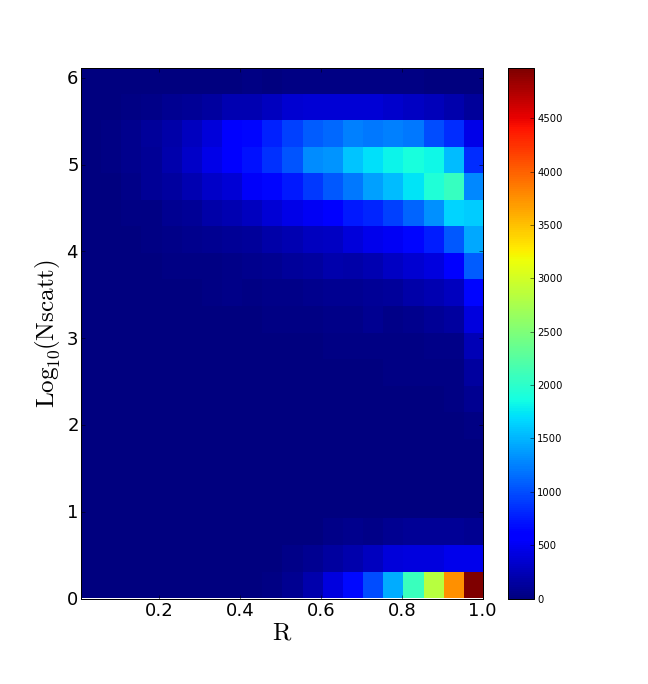
\includegraphics[scale=0.6]{Histogram2dNscattVSRadius.png}
\end{center}
\caption{\label{nscatt} 2D histogram of the number of scatterings and
  the number. The color scale is linear in the number of photons in
  each bin.}
\end{figure}


\subsection*{End of paragraph 3.3}

{\bf One sentence is not clear : we see that the escape fraction does
  not increase significantly from $\tau$ = 105 to $\tau =
  10^{6}$. This counter-intuitive result.... It sounds like you were
  expecting a strong increase... A decrease is expected from $\tau$ =
  105 to $\tau$ = 106, not an increase, but indeed on the graphe we
  can see an unexpected (small) increase. I do not understand the
  explanation for this behaviour.} 


(MARK)

\subsection*{Fig8}


{\bf Referred to as Figure 7 in the text (paragraph 3.4). To my mind,
  this figure illustrates the main result of your study, it has to be
  more demonstrative. On this figure, the numerical noise seems very
  big compare to the small number of bins, bigger than on the spectra
  from Fig1, how is it possible ? Could you re-do this figure with
  more photons, maybe with more bins ? Could you plot an histogram
  instead of broken lines, to ease the reading ? In the text, you
  write anisotropy induced by rotation is at the 3$\%$ level, how do
  to estimate this number? I think that the noise is at $3\%$ level,
  and the distribution is compatible with ’flat’. In the corresponding
  text, you first say that $F(\mu)$ does not depend on Vmax. Again, if
  real, this is an important result, that you must advertise
  more. Please show it on this Fig, by comparing F($\mu$) without rotation
  (in red, for example) to the other distributions that you get with
  different values of Vmax. Then, you mention that for high optical
  depth values, $F(\mu)$ (not the variations of $\mu$) can vary up to
  $15\%$. First, what do you call high optical depth ? your highest
  setup is $\tau$= $10^7$, not extremely high for lyman alpha ”standards’,
  corresponding to NHI $\sim$10$^{20}$ cm$^{-2}$. So, if you see a trend with
  optical depth, I encourage you to check higher optical depth
  regimes, corresponding better to galaxy scales. If you can probe
  that anisotropy induced by rotation is rising with optical depth,
  this would be an interesting result. If higher optical depth regimes
  lead to anisotropic escape, could you check the effet of anisotropy
  on the lya spectral shape?} 


We have prepared Figure 5 that shows the $F(\mu)$ distribution for
different velocities and optical depths. Indeed, the distributions are
consistent with flat (within the noise levels) for all the models
studied in our paper. 

We did not try many more models with higher optical depths. We expect
to do that in the near future to complete a study that could be
immediatly comparable against observations.




\end{document}
